\subsection{Visitor Pattern und Double Dispatch}


\subsubsection*{Problembeschreibung}

Gelegentlich muss eine Operation auf einer Menge von Objekten durchgeführt, die zwar all Teil einer Aggregationshiearchie aber dennoch unterschiedlich sind.  Diese Objekte besitzen unter Umständen voneinander abweichende Interfaces. Das Visitor-Pattern erlaubt es, solche Operationen außerhalb der Objekte und für alle betroffenen Objekte innerhalb einer Klasse zu definieren.

\subsubsection*{Lösung}

Der konkrete Visitor realisiert das Visitor-Interface, welches die Methode `visit` bereitstellt. Diese erlaubt es dem Visitor, ein Element zu "besuchen" und auf ihm eine Operation durchzuführen. Die Elemente "akzeptieren" den "Besuch" des Visitors mit Hilfe der Methode `accept`, welche als Argument den besuchenden Visitor erhält.

\begin{figure}[!hb]
	\centering
	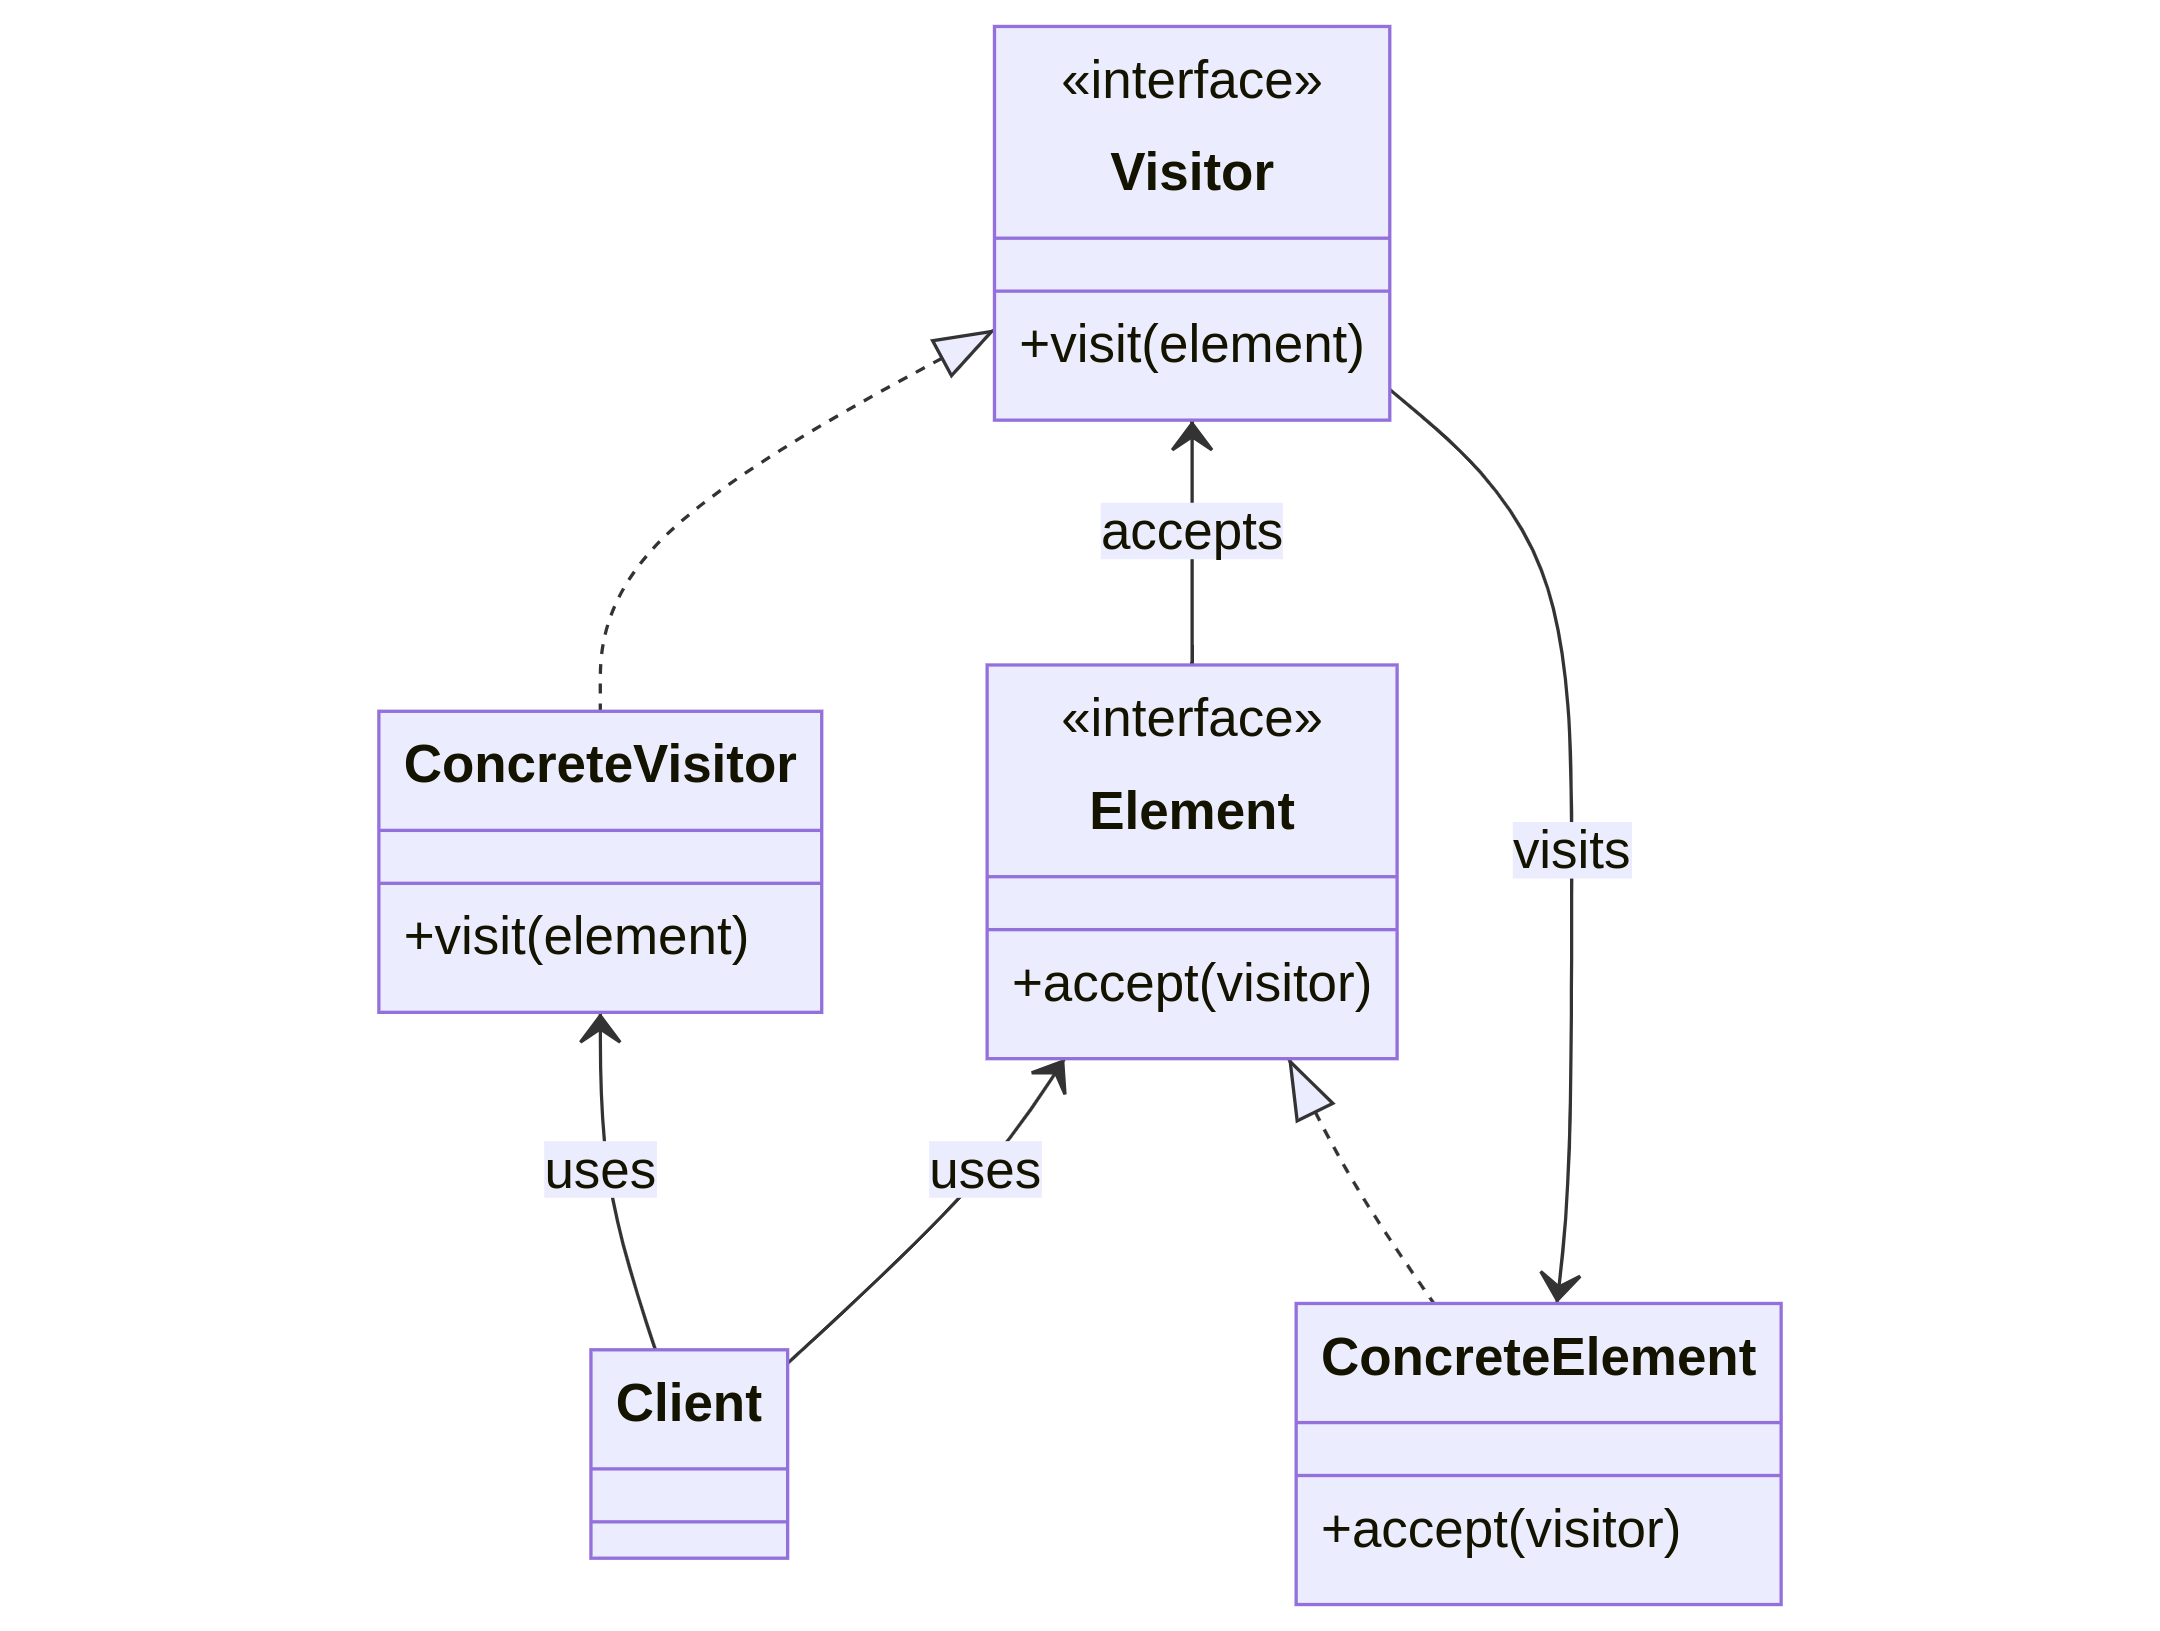
\includegraphics[width=0.75\linewidth]{images/patterns/visitor-class.png}
	\caption{Klassendiagramm Visitor}
	\label{fig:visitor-class}
\end{figure}

Der Client trägt dem Visitor auf, eine Operation auf einem Element oder einer Menge von Elementen durchzuführen (1). Der Visitor sendet daraufhin `visit` an alle Elemente, auf die er eine Referenz hält (2). Jedes Element ruft daraufhin eine `accept`-Methode auf dem Visitor auf. Zu beachten ist hierbei, dass es für jede Element-Klasse eine eigene Methode im Visitor gibt. Dies kann realisiert werden durch das Bereitstellen von Methoden mit unterschiedlichen, zu den aufrufenden Klassen korrespondierenden Namen oder durch Multimethoden. Multimethoden sind Methoden, welche je nach Typ der übergebenen Argumente unterschiedliche Implementierungen ausführen. Somit kann der Visitor nach Erhalt von `accept` die zum Typ des sendenden Elements passende Operation ausführen. Dieser Mechanismus nennt sich **Double-Dispatch**. 

\begin{figure}[!hb]
	\centering
	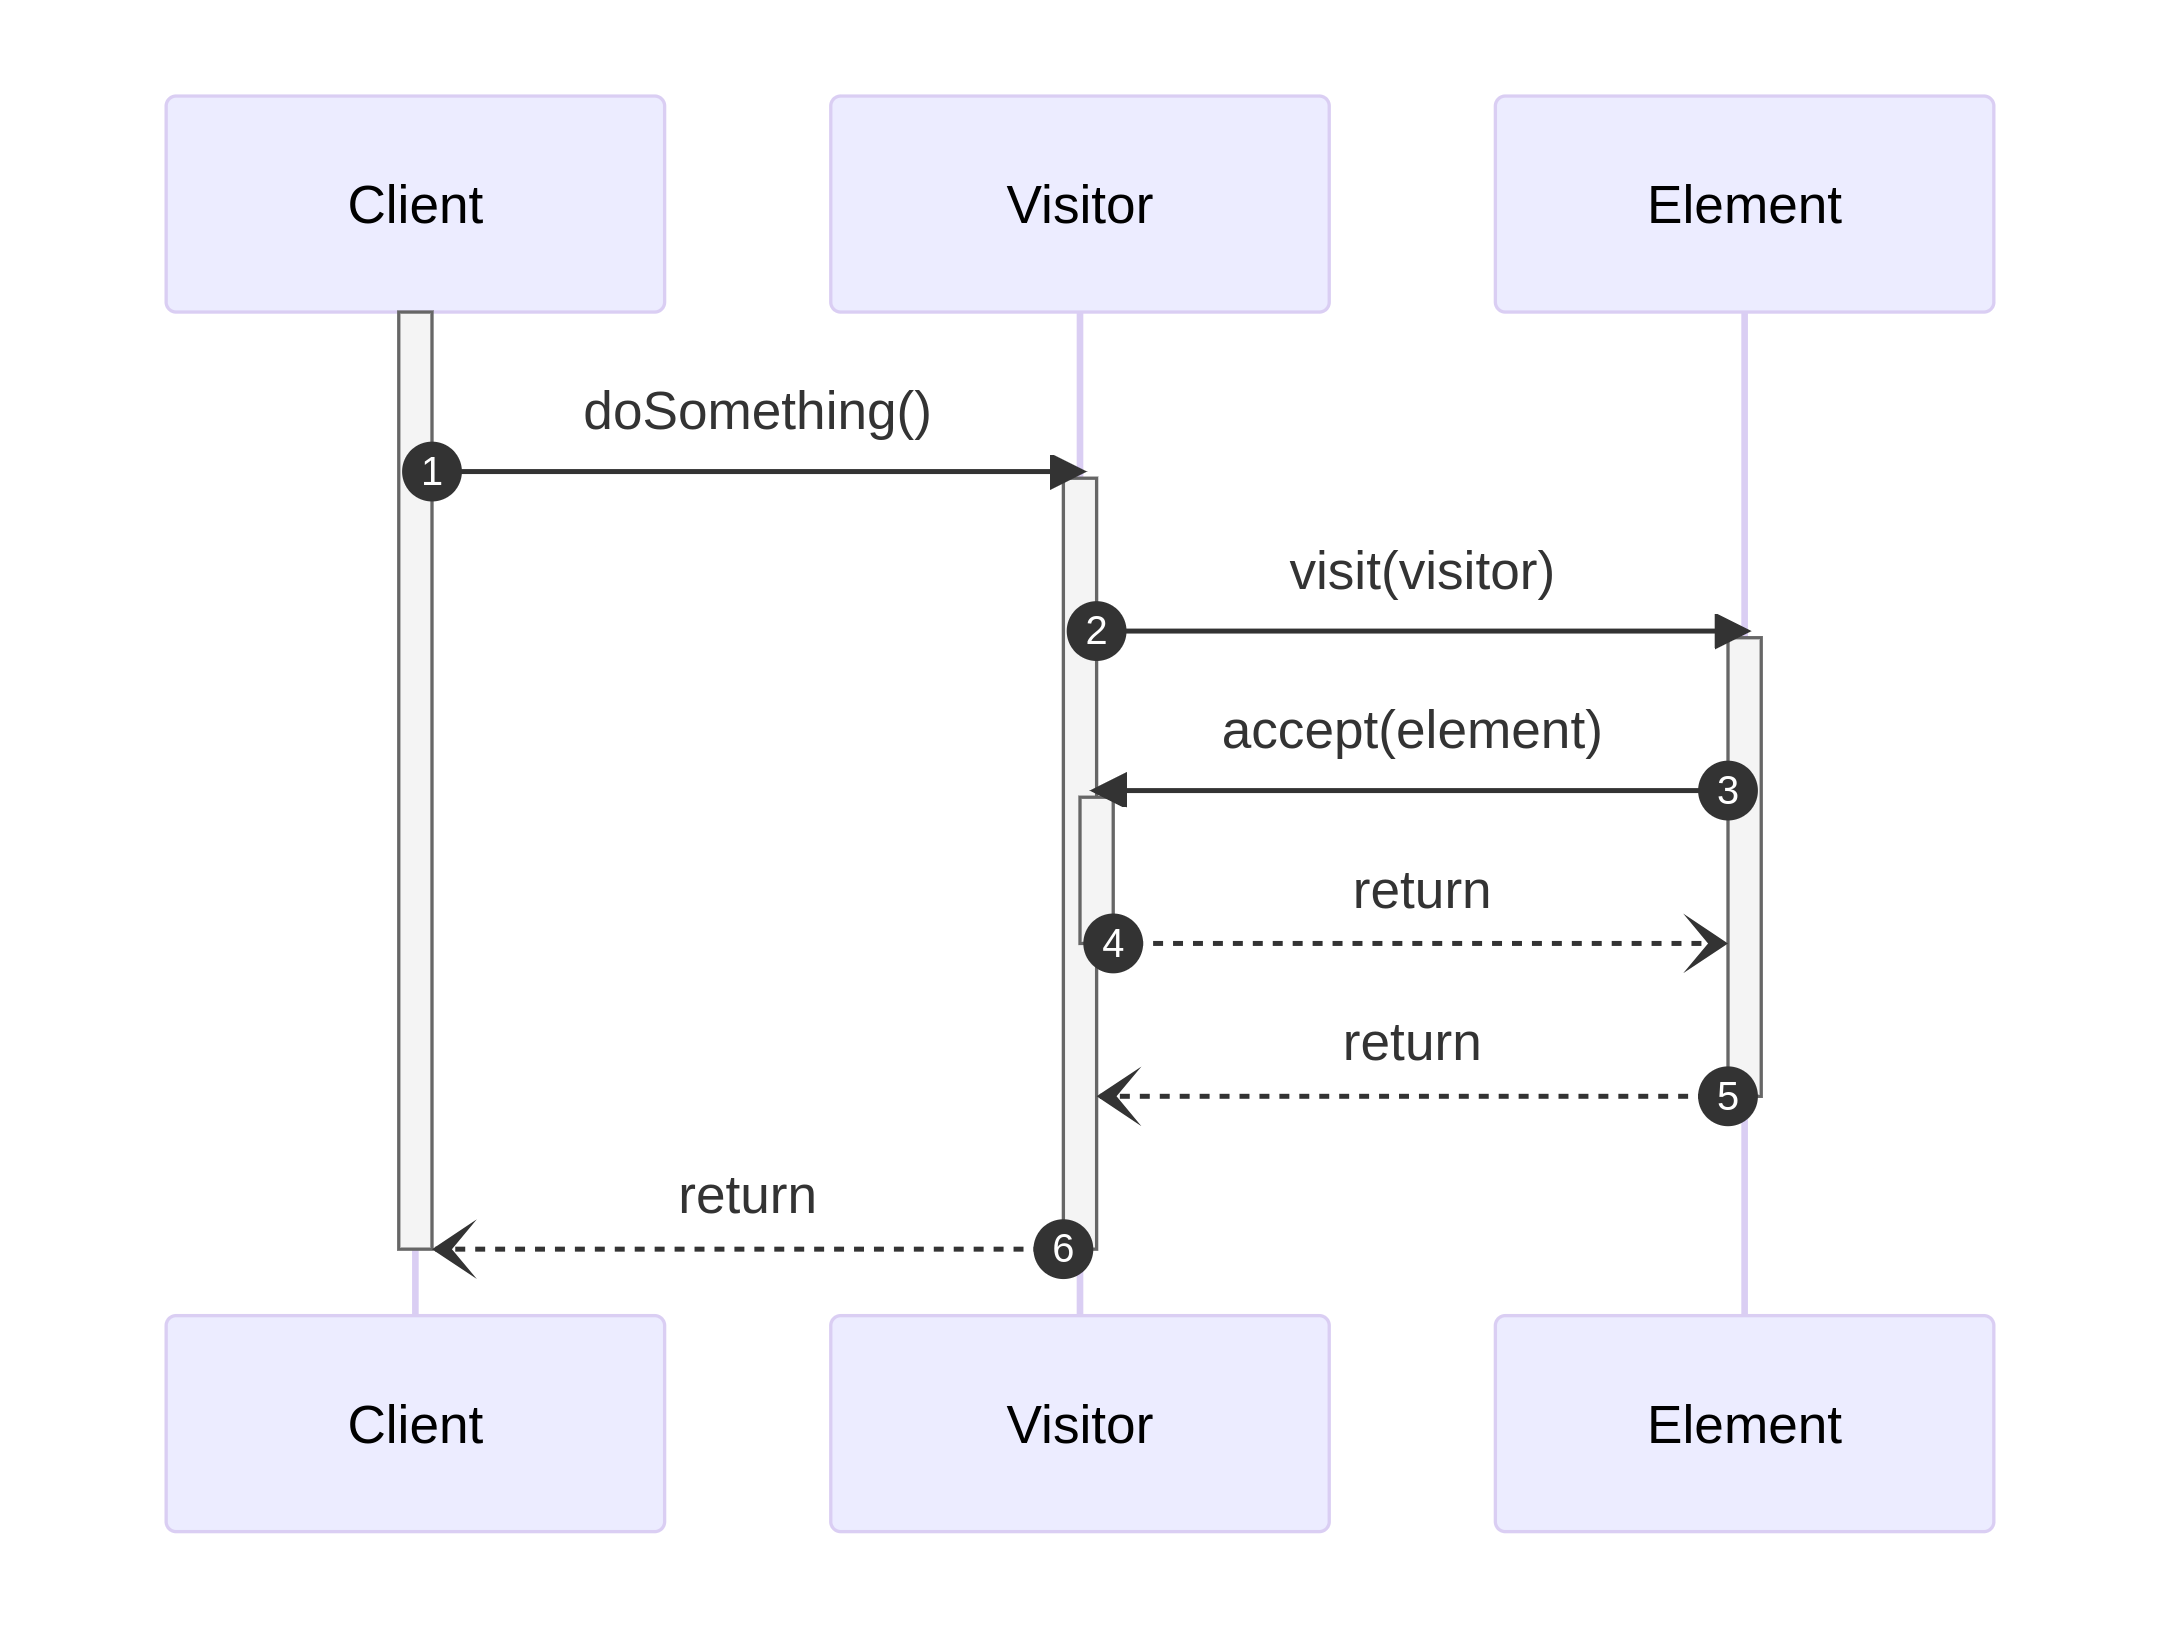
\includegraphics[width=0.75\linewidth]{images/patterns/visitor-seq.png}
	\caption{Sequenzdiagramm Visitor}
	\label{fig:visitor-seq}
\end{figure}

\subsubsection*{Konsequenzen}
Durch die Kapselung der Operation in einem Visitor, ist es sehr einfach, neue Operationen hinzuzufügen. Es bedarf dazu lediglich eines weiteren Visitors. Außerdem kapselt ein Visitor die Menge an Operationen auf den Elementen. Zusammengehörige Operationen werden in einer Klasse gesammelt. Nicht zueinander gehörende Operationen befinden sich in unterschiedlichen Visitors. Ein weiterer Vorteil eines Visitors ist dessen Fähigkeit, während des "Besuchens" mehrerer Elemente Informationen über diese zu akkumulieren und im Anschluss gebündelt zu repräsentieren. 

Der Visitor weist jedoch auch Nachteile auf. Zum einen ist es schwer, weitere konkrete Element-Klassen zu einem System hinzuzufügen, welches bereits eine Reihe an Visitors besitzt. Da ein Visitor für jeden Typ von Element eine Methode bereitstellen muss, kann ein  weiteres Element einen erhöhten Implementierungsaufwand bedeuten. Das Visitor-Pattern sollte daher nur verwendet werden, wenn entweder die Menge an Elementklassen abgeschlossen oder die Menge an Visitor-Klassen übersichtlich ist. Weiterhin müssen die Elemente dem Visitor ein Interface bereitstellen, welches es dem Visitor ermöglicht, seine Operation ausführen zu können. Dies kann dazu führen, dass das Element einen großen Teil seines internen Zustands preisgeben muss, welcher bei nicht-Verwendung dieses Patterns gekapselt geblieben wäre.